\section{Multiplier/diviser un nombre décimal par 10, 100, 1000}
%%%%%%%%%%%%%%%%%%%%%%%%%%%%%%%%%%%%%%%%%%%%%%%%%%%%%%%%%%%%%%%%%%%%%%%%%%%
\prof
{En primaire et de façon usuelle, on a l'habitude de parler de virgule qui se déplace. Cependant, pour coller à la réalité mathématiques, on préférera ici parler de quantité qui augment ou qui diminue et donc de chiffres qui se déplacent. Cela n'empêche pas, une fois le concept acquis de montrer qu'on peut imaginer un déplacement de la virgule.}
%%%%%%%%%%%%%%%%%%%%%%%%%%%%%%%%%%%%%%%%%%%%%%%%%%%%%%%%%%%%%%%%%%%%%%%%%%%

\begin{aconnaitre}

\hspace{2em}\textbullet\hspace{.25em} Multiplier un nombre décimal par 10, 100 ou 1 000 revient à \textbf{\textcolor{C2}{déplacer chacun de ses chiffres vers la gauche}} de 1, 2 ou 3 rangs pour lui donner une valeur 10, 100 ou 1 000 fois plus grande.

\hspace{2em}\textbullet\hspace{.25em} Diviser un nombre décimal par 10, 100 ou 1 000 revient à \textbf{\textcolor{C2}{déplacer chacun de ses chiffres vers la droite}} de 1, 2 ou 3 rangs pour lui donner une valeur 10, 100 ou 1 000 fois plus petite.

\end{aconnaitre}

\begin{methode*1}[]
	\begin{remarque}
On devra parfois ajouter des zéros dans l'écriture.
	\end{remarque}
	\begin{exemple*1}

Effectuer les calculs $6,5 \div 100$ et $0,47 \times 1000$ [0.5em]

\begin{minipage}{.4\linewidth}
\begin{ttableau}{.8\linewidth}{4}
\hline
 \rotatebox{90}{unités} & \rotatebox{90}{dixièmes} & \rotatebox{90}{centièmes\phantom{x}} & \rotatebox{90}{millièmes} \\ \hline
 \textcolor{B1}{\textbf{6}} , & \textcolor{B1}{\textbf{5}} & & \\ \hline
 $0\,,$ & 0 & \textcolor{B1}{\textbf{6}} & \textcolor{B1}{\textbf{5}} \\ \hline
\end{ttableau}
\end{minipage}\hfill%
%
\begin{minipage}{.55\linewidth}
Pour diviser 6,5 par \textcolor{B1}{\textbf{100}}, on déplace chacun de ses chiffres vers la droite de \textcolor{B1}{\textbf{2}} rangs et on ajoute les zéros nécessaires. 

On obtient $6,5 \div 100 = 0,065$.

\end{minipage}
%

\vspace{2em}

\begin{minipage}{.4\linewidth}
\begin{ttableau}{\linewidth}{5}
\hline
\rotatebox{90}{centaines} & \rotatebox{90}{dixaines} & \rotatebox{90}{unités} & \rotatebox{90}{dixièmes} & \rotatebox{90}{centièmes\phantom{x}} \\ \hline
 & & 0 , & \textcolor{J1}{\textbf{4}} & \textcolor{J1}{\textbf{7}} \\ \hline
 \textcolor{J1}{\textbf{4}} & \textcolor{J1}{\textbf{7}} & 0 & &\\ \hline
\end{ttableau}
\end{minipage}\hfill%
%
\begin{minipage}{.55\linewidth}
Pour multiplier 0,47 par \textcolor{J1}{\textbf{1\,000}}, on déplace chacun de ses chiffres vers la gauche de \textcolor{J1}{\textbf{3}} rangs et on ajoute les zéros nécessaires. 

On obtient $0,47 \times 1\,000 = 470$. 
\end{minipage}
	\end{exemple*1}
	
\exercice

Compléter par le signe qui convient.
\begin{colenumerate}{4}
 \item $0,8 \dotfill 100=80$ ;
 \item $0,38 \dotfill 10=0,038$ ;
 \item $47 \dotfill 100=0,47$ ;
 \item $5 \dotfill 0,1=0,5$;
 \end{colenumerate}


\exercice

Effectue : 
\begin{colenumerate}{4}
 \item $3,6 \times 100$ ;
 \item $870 \times 1\,000$ ;
 \item $63 \div 10$ ;
 \item $87\,654 \div 100$.
 \end{colenumerate}
%\correction
 
\end{methode*1}








%%%%%%%%%%%%%%%%%%

\section{Multiplier/diviser un nombre décimal par 0,1 ; 0,01 ; 0,001}

\begin{aconnaitre}
\textbf{Multiplier} un nombre décimal par \textcolor{A1}{\textbf{0,1}}, \textcolor{B1}{\textbf{0,01}} ou \textcolor{J1}{\textbf{0,001}} revient à déplacer chacun de ses chiffres vers \textbf{la droite} de 1, 2 ou \textcolor{J1}{\textbf{3}} rangs pour lui donner une valeur 10, 100 ou \textcolor{J1}{\textbf{1\,000}} fois plus petite.
\textbf{Diviser} un nombre décimal par \textcolor{A1}{\textbf{0,1}}, \textcolor{B1}{\textbf{0,01}} ou \textcolor{J1}{\textbf{0,001}} revient à déplacer chacun de ses chiffres vers \textbf{la gauche} de \textcolor{A1}{\textbf{1}}, \textcolor{B1}{\textbf{2}} ou \textcolor{J1}{\textbf{3}} rangs pour lui donner une valeur \textcolor{A1}{\textbf{10}}, \textcolor{B1}{\textbf{100}} ou \textcolor{J1}{\textbf{1\,000}} fois plus grande.
\end{aconnaitre}


\begin{methode*1}[Multiplier ou diviser un nombre décimal par 0,1 ; 0,01 ; 0,001 \ldots]

\begin{remarque}
On devra parfois ajouter des zéros dans l'écriture.
\end{remarque}

\begin{exemple*1}
Effectue les calculs $2,5 \times 0,01$ et $0,65 \div 0,001$.\\[1em]

\begin{minipage}{.4\linewidth}
\begin{ttableau}{.8\linewidth}{4}
\hline
 \rotatebox{90}{unités} & \rotatebox{90}{dixièmes} & \rotatebox{90}{centièmes\phantom{x}} & \rotatebox{90}{millièmes} \\ \hline
 \textcolor{B1}{\textbf{2}} , & \textcolor{B1}{\textbf{5}} & & \\ \hline
 $0\,,$ & 0 & \textcolor{B1}{\textbf{2}} & \textcolor{B1}{\textbf{5}} \\ \hline
\end{ttableau}
\end{minipage}\hfill%
%
\begin{minipage}{.55\linewidth}
Pour multiplier 2,5 par \textcolor{B1}{\textbf{0,01}}, on déplace chacun de ses chiffres vers la droite de \textcolor{B1}{\textbf{2}} rangs et on ajoute les zéros nécessaires. 

On obtient $2,5 \times 0,01 = 0,025$.
\end{minipage}
%

\vspace{2em}

%
\begin{minipage}{.4\linewidth}
\begin{ttableau}{\linewidth}{5}
\hline
\rotatebox{90}{centaines} & \rotatebox{90}{dixaines} & \rotatebox{90}{unités} & \rotatebox{90}{dixièmes} & \rotatebox{90}{centièmes\phantom{x}} \\ \hline
 & & 0 , & \textcolor{J1}{\textbf{6}} & \textcolor{J1}{\textbf{5}} \\ \hline
 \textcolor{J1}{\textbf{6}} & \textcolor{J1}{\textbf{5}} & 0 & &\\ \hline
\end{ttableau}
\end{minipage}\hfill%
%
\begin{minipage}{.55\linewidth}
Pour diviser 0,65 par \textcolor{J1}{\textbf{0,001}}, on déplace chacun de ses chiffres vers la gauche de \textcolor{J1}{\textbf{3}} rangs et on ajoute les zéros nécessaires. 

On obtient $0,65 \div 0,001 = 650$.
\end{minipage}
\end{exemple*1}


\exercice

Effectuer :
\begin{colenumerate}{4}
 \item $5,45 \times 0,1$ ;
 \item $854 \times 0,001$ ;
 \item $63 \div 0,1$ ;
 \item $87,54 \div 0,01$.
 \end{colenumerate}
%\correction

\end{methode*1}

%%%%%%%%%%%%%%%%%%%%%%%%%%%%%%%%%%%%%%%%%%%%%%%%%%%%%%%%
\section{Multiplication}
\begin{remarque}

Multiplier c'est répéter la même quantité un certain nombre de fois.
\end{remarque}
	\subsection{Multiplier des décimaux}
\begin{aconnaitre}
Le résultat d'une multiplication s'appelle un produit. Les nombres que l'on multiplie sont des facteurs.
\end{aconnaitre}

\begin{methode*1}[Multiplication]
\begin{exemple*1}

$12 \times 4=48$

48 est le produit. 12 et 4 sont des facteurs.
\end{exemple*1}

\exercice

$13\times 3=39$

\dotfill est le \dotfill . \dotfill et \dotfill sont des \dotfill .

\end{methode*1}

	\subsection{Multiplier plusieurs facteurs}
\begin{aconnaitre}
Dans le calcul d'un produit de plusieurs facteurs, on peut:

\hspace{2em}\textbullet\hspace{.25em} changer l'ordre des facteurs.

\hspace{2em}\textbullet\hspace{.25em} regrouper différemment certains facteurs pour faciliter les calculs.
\end{aconnaitre}
\begin{methode*1}[]
\begin{exemple*1}

$25 \times 32 \times 4=25 \times 4 \times 32=100  \times 32 = 3200$
\end{exemple*1}

\exercice

$2 \times 3 \times 5= \dotfill$
\end{methode*1}
	
	\subsection{Multiplier deux nombres décimaux}
\begin{methode*1}[Multiplication de décimaux]
\begin{exemple*1}

Effectue la multiplication de 2,34 par 1,2.\\[0.5em]

On pose l'opération comme s'il s'agissait de nombres entiers. 

On effectue la multiplication de 234 par 12 sans tenir compte des virgules.

\begin{minipage}{.6\linewidth}
\begin{tabular}{rrrrcrrrr}
& 2, & 3 & 4 & $\xrightarrow{\times \text{\textcolor{B1}{\textbf{100}}}}$ & & 2 & 3 & 4 \\
$\times$ & & 1, & 2 & $\xrightarrow{\times \text{\textcolor{A1}{\textbf{10}}}}$ & $\times$ & & 1 & 2 \\ \cline{1-4} \cline{6-9}
& & & & & & 4 & 6 & 8 \\
& & & & & 2 & 3 & 4 & . \\ \cline{1-4} \cline{6-9}
2, & 8 & 0 & 8 & $\xleftarrow{\,\div\,\text{\textcolor{J1}{\textbf{1\,000}}}}$ & 2 & 8 & 0 & 8 \\
\end{tabular}
\end{minipage}\hfill%
%
\begin{minipage}{.37\linewidth}
234 est \textcolor{B1}{\textbf{100}} fois plus grand que 2,34 et 12 est \textcolor{A1}{\textbf{10}} fois plus grand que 1,2. Le produit $2,34 \times 1,2$ est donc \textcolor{J1}{\textbf{1\,000}} fois plus petit que 2\,808. Pour obtenir le résultat, on effectue donc $2\,808 \div 1\,000$.\\[0.75em]
\end{minipage}
Finalement $2,34 \times 1,2 = 2,808$.
\end{exemple*1}

\exercice

Sachant que $168 \times 32 = 5\,376$, détermine les produits (sans aucun calcul) :
\begin{colenumerate}{4}
 \item $168 \times 3,2$ ;
 \item $16,8 \times 0,32$ ;
 \item $1\,680 \times 3,2$ ;
 \item $1,68 \times 32$.
\end{colenumerate}
%\correction

Pose et effectue les opérations :
\begin{colenumerate}{4}
 \item $68,7 \times 39$ ;
 \item $123 \times 6,3$ ;
 \item $1,3 \times 0,7$ ;
 \item $54,6 \times 8,25$.
\end{colenumerate}
%\correction
\end{methode*1}

%%%%%%%%%%%%%%%%%%%%%%%%%%%%%%%%%%%%%%%%%%%%%%%%%%%%%%%%%%%%%%%%%%%%%%%%%%%  
\section{Division}
\begin{remarque}

Diviser c'est:
\begin{itemize}
\item partager une quantité en parts égales\\
OU
\item constituer des groupes de même taille
\end{itemize}
\end{remarque}
\begin{methode*1}[Diviser un nombre décimal par un nombre entier]

\begin{exemple*1}
Effectue la division de 75,8 par 4.\\[0.5em]

\begin{minipage}[c]{.26\textwidth}
\vspace{0em}
\begin{center}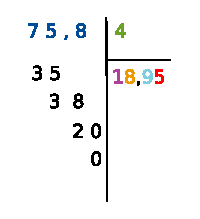
\includegraphics[width=3cm]{div758-4} \end{center}

\end{minipage}\hfill% 
\begin{minipage}[c]{.66\textwidth}

On commence par diviser la partie entière. On partage \textcolor{A1}{7} dizaines en \textcolor{H1}{4} ; le quotient comportera \textcolor{C1}{1} dizaine.\\[0.75em]
Il reste 3 dizaines. Avec les \textcolor{A1}{5} unités en plus, cela fait 35 unités à partager en \textcolor{H1}{4} ; le quotient comportera \textcolor{J1}{8} unités. \\[0.75em]
Il reste 3 unités soit 30 dixièmes. Avec les \textcolor{A1}{8} dixièmes en plus, cela fait 38 dixièmes à partager en \textcolor{H1}{4} ; le quotient comportera \textcolor{A3}{9} dixièmes. On doit donc écrire la virgule dans le quotient.\\[0.75em]
Il reste 2 dixièmes soit 20 centièmes (on a ajouté un zéro) à partager en \textcolor{H1}{4} ; le quotient comportera donc \textcolor{B2}{5} centièmes.\\[0.75em]
Ainsi $\textcolor{A1}{75,8} \div \textcolor{H1}{4} = \textcolor{C1}{1}\textcolor{J1}{8},\textcolor{A3}{9}\textcolor{B2}{5}$.
\end{minipage}

\end{exemple*1}

\exercice

Calcule la valeur exacte ou une valeur arrondie au centième des quotients :
\begin{colenumerate}{4}
 \item $10 \div 7$ ;
 \item $24,96 \div 8$ ;
 \item $5,2 \div 6$ ;
 \item $145,2 \div 3$.
 \end{colenumerate}
%\correction

\end{methode*1}

%%%%%%%%%%%%%%%%%%%%%%%%%%%%%%%%%%%%%%%%%%%%%%%%%%%%%%%%%%%%%%%%%%%%%%%%%%%

\begin{aconnaitre}
Le quotient de deux nombres \textbf{ne change pas} si on les multiplie (le dividende et le diviseur) par un même nombre non nul.
\end{aconnaitre}


\begin{methode*1}[Diviser un nombre décimal par un nombre décimal]

\begin{exemple*1}
Effectue la division de 32,4 par 2,25.\\[1em]
On commence par rendre entier le diviseur en le multipliant par 100 : $2,25 \times 100 = 225$. On multiplie le dividende par le même nombre : $32,4 \times 100 = 3\,240$. On effectue la division de 3\,240  par 226, soit $3\,240 \div 225 = 14,4$. On obtient ainsi le résultat de la division :

$32,4 \div 2,25 = 14,4$. 
\end{exemple*1}

\exercice

Calcule la valeur exacte ou une valeur arrondie au centième des quotients :
\begin{colenumerate}{4}
 \item $4 \div 6,37$ ;
 \item $13,4 \div 2,45$ ;
 \item $5,87 \div 2,3$ ;
 \item $0,84 \div 0,12$.
 \end{colenumerate}
%\correction

\end{methode*1}

%%%%%%%%%%%%%%%%%%%%%%%%%%%%%%%%%%%%%%%%%%%%%%%%%%%%%%%%%%%%%%%%%%%%%%%%%%%        

